

\chapter{Double Scenario Classification of the first and last shared app, KFold Validation}

Starting with fitting randomly the classifiers, there are some statistics of the data used for the first test: \\
 {\def\arraystretch{1.3} 
 \begin{table}[H] 
\centering 
\begin{tabular}{|l|l|l|} 
\hline 
  &count train  &count test  \\ \hline
mess\_mess  &96  &254  \\ \hline
tele\_mess  &99  &251  \\ \hline
what\_mess  &107  &243  \\ \hline
mess\_tele  &98  &252  \\ \hline
tele\_tele  &111  &239  \\ \hline
what\_tele  &105  &245  \\ \hline
mess\_what  &116  &234  \\ \hline
tele\_what  &103  &247  \\ \hline
what\_what  &121  &229  \\ \hline
original  &94  &256  \\ \hline
\end{tabular} 
\end{table} }
\section{Logistic regression results:} 
Confusion matrix with number of sample and with normalization:
 {\def\arraystretch{1.3} 
 \begin{table}[H] 
\centering 
\begin{tabular}{|l|l|l|l|l|l|l|l|l|l|l|} 
\hline 
  &m\_m  &m\_t  &m\_w  &t\_m  &t\_t  &t\_w  &w\_m  &w\_t  &w\_w  &original  \\ \hline
mess\_mess  &249  &4  &1  &0  &0  &0  &0  &0  &0  &0  \\ \hline
tele\_mess  &0  &241  &9  &0  &1  &0  &0  &0  &0  &0  \\ \hline
what\_mess  &21  &9  &213  &0  &0  &0  &0  &0  &0  &0  \\ \hline
mess\_tele  &0  &0  &1  &43  &107  &2  &0  &99  &0  &0  \\ \hline
tele\_tele  &0  &0  &0  &52  &79  &0  &0  &108  &0  &0  \\ \hline
what\_tele  &0  &0  &0  &0  &1  &243  &0  &1  &0  &0  \\ \hline
mess\_what  &0  &2  &0  &0  &0  &0  &84  &2  &146  &0  \\ \hline
tele\_what  &0  &0  &0  &57  &112  &0  &0  &78  &0  &0  \\ \hline
what\_what  &0  &0  &0  &0  &0  &0  &102  &0  &124  &3  \\ \hline
original  &1  &0  &0  &0  &0  &0  &0  &0  &4  &251  \\ \hline
\end{tabular} 
\end{table} }

 \begin{figure}[H] 
\centering 
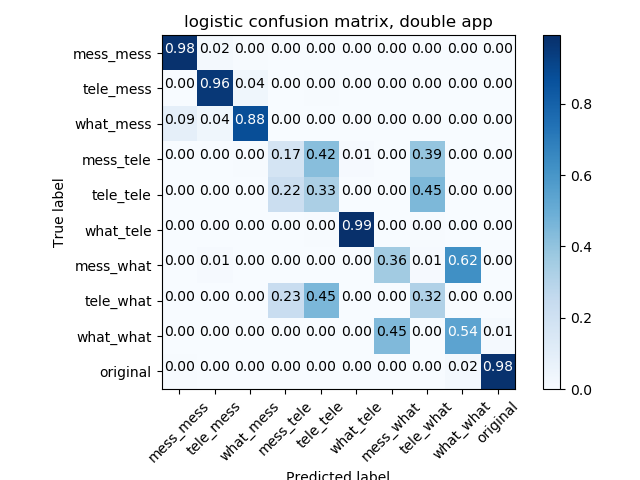
\includegraphics[scale=.6]{images/lr_initial_double_complete.png} 
\caption{logistic regression, last app classified} 
\end{figure} 


Result of the KFold validation with 10 bins:
 {\def\arraystretch{1.3} 
 \begin{table}[H] 
\centering 
\begin{tabular}{|l |l |l |l |l |l |l |l |l |l |}  
\hline 
0.5905&
0.5905&
0.6571&
0.6190&
0.5810&
0.6476&
0.7048&
0.6762&
0.6190&
0.6762\\ \hline  

\end{tabular} 
\end{table} }

The mean is : 0.636190\section{Linear Support Vector Machine results:} 
Confusion matrix with number of sample and with normalization:
 {\def\arraystretch{1.3} 
 \begin{table}[H] 
\centering 
\begin{tabular}{|l|l|l|l|l|l|l|l|l|l|l|} 
\hline 
  &m\_m  &m\_t  &m\_w  &t\_m  &t\_t  &t\_w  &w\_m  &w\_t  &w\_w  &original  \\ \hline
mess\_mess  &246  &3  &2  &0  &0  &0  &2  &0  &0  &1  \\ \hline
tele\_mess  &0  &233  &9  &0  &4  &0  &2  &0  &3  &0  \\ \hline
what\_mess  &22  &5  &209  &3  &0  &4  &0  &0  &0  &0  \\ \hline
mess\_tele  &0  &0  &0  &47  &102  &1  &0  &101  &1  &0  \\ \hline
tele\_tele  &0  &0  &0  &55  &58  &4  &0  &122  &0  &0  \\ \hline
what\_tele  &0  &0  &0  &1  &0  &244  &0  &0  &0  &0  \\ \hline
mess\_what  &0  &1  &0  &0  &0  &0  &90  &2  &141  &0  \\ \hline
tele\_what  &0  &0  &0  &58  &108  &3  &0  &78  &0  &0  \\ \hline
what\_what  &0  &0  &0  &0  &0  &0  &114  &0  &112  &3  \\ \hline
original  &0  &0  &0  &0  &1  &0  &1  &0  &8  &246  \\ \hline
\end{tabular} 
\end{table} }

 \begin{figure}[H] 
\centering 
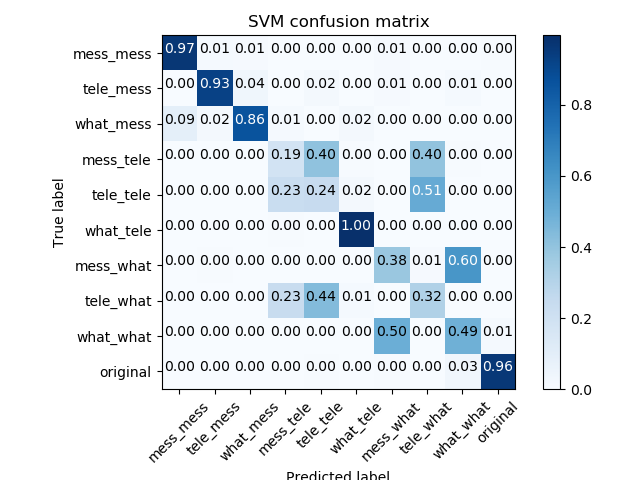
\includegraphics[scale=.6]{images/lsvm_initial_double_complete.png} 
\caption{linear SVM, last app classified} 
\end{figure} 


Result of the KFold validation with 10 bins:
 {\def\arraystretch{1.3} 
 \begin{table}[H] 
\centering 
\begin{tabular}{|l |l |l |l |l |l |l |l |l |l |}  
\hline 
0.5905&
0.5619&
0.6857&
0.6000&
0.5429&
0.6286&
0.6762&
0.6667&
0.5810&
0.6571\\ \hline  

\end{tabular} 
\end{table} }

The mean is : 0.619048\section{Random forest results:} 
Confusion matrix with number of sample and with normalization:
 {\def\arraystretch{1.3} 
 \begin{table}[H] 
\centering 
\begin{tabular}{|l|l|l|l|l|l|l|l|l|l|l|} 
\hline 
  &m\_m  &m\_t  &m\_w  &t\_m  &t\_t  &t\_w  &w\_m  &w\_t  &w\_w  &original  \\ \hline
mess\_mess  &244  &6  &3  &0  &0  &0  &1  &0  &0  &0  \\ \hline
tele\_mess  &1  &243  &7  &0  &0  &0  &0  &0  &0  &0  \\ \hline
what\_mess  &24  &18  &193  &0  &0  &0  &2  &0  &5  &1  \\ \hline
mess\_tele  &0  &0  &0  &35  &109  &3  &0  &105  &0  &0  \\ \hline
tele\_tele  &0  &0  &0  &81  &39  &4  &0  &115  &0  &0  \\ \hline
what\_tele  &0  &0  &0  &1  &0  &243  &0  &1  &0  &0  \\ \hline
mess\_what  &0  &1  &0  &0  &0  &0  &62  &0  &171  &0  \\ \hline
tele\_what  &0  &0  &0  &80  &121  &5  &0  &41  &0  &0  \\ \hline
what\_what  &0  &0  &0  &0  &0  &0  &123  &0  &103  &3  \\ \hline
original  &0  &0  &1  &0  &0  &0  &0  &0  &2  &253  \\ \hline
\end{tabular} 
\end{table} }

 \begin{figure}[H] 
\centering 
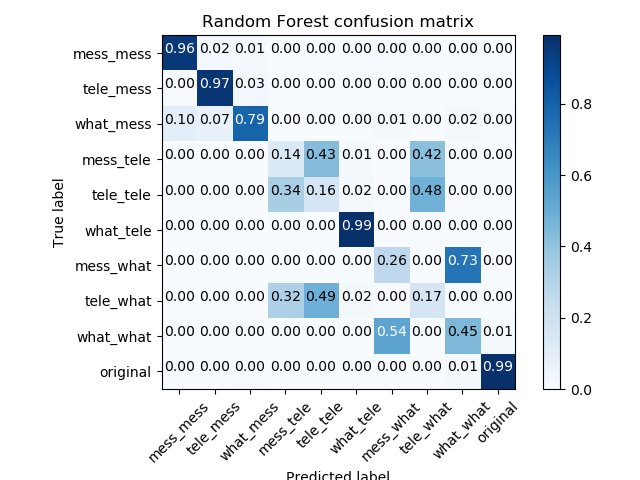
\includegraphics[scale=.6]{images/rf_initial_double_complete.png} 
\caption{random forest, last app classified} 
\end{figure} 


Result of the KFold validation with 10 bins:
 {\def\arraystretch{1.3} 
 \begin{table}[H] 
\centering 
\begin{tabular}{|l |l |l |l |l |l |l |l |l |l |}  
\hline 
0.5905&
0.5048&
0.6095&
0.6000&
0.5524&
0.6286&
0.6095&
0.6286&
0.5238&
0.6000\\ \hline  

\end{tabular} 
\end{table} }

The mean is : 0.58476229